\chapter{Research}
\label{research}

\section{Data selection}
\label{method:data}
A total number of 250 OSS projects will be used for this study. This number is
somewhat arbitrary, but was chosen to have a larger data set than the initial
study conducted by \citet{karus2013}, as a larger data set yields more
trustworthy results. However, the research still needs to be feasible within
the given time constraints of four months.

Several steps have been taken prior to the selection of this set of 250
projects. The steps are described in the following sections.

\subsection{Data gathering}
The data for this research is gathered from
Ohloh\footnote{\url{http://www.ohloh.net}}: \textit{``Ohloh is a free, public
directory of Free and Open Source Software and the contributors who create and
maintain it.'' } \cite{ohloh}. At the time of this writing, Ohloh tracks more
than 660,000 OSS projects varying in all ranges of size, and popularity. The
most popular projects currently being Apache HTTP Server, Apache OpenOffice,
Apache Subversion, Bash, Firebug, Linux Kernel, Mozilla Firefox, MySQL, PHP,
and Ubuntu.

\paragraph{}
For this research, the data provided by a tool by \citet{ohlohanalytics} is
used. This tool, ``\textit{OhlohAnalytics}'', was developed as part of the
replication research by \citet{bruntink2013}, and provides a validated and
cleansed data set of 12,360 OSS projects, collected from Ohloh in July 2013.

\subsubsection{Initial validation and cleansing}
The OhlohAnalytics tool performed initial analysis, validation, and cleansing
of the data by detecting inconsistent values and removing these records from
the data set. Additionally, extra data fields are derived or aggregated from
and added to the raw data for convenience.

The complete list of data fields provided by OhlohAnalytics is shown in Table
\ref{table:fields}. The column 'Source' specifies if the field is either 'Raw'
data (i.e., directly available from Ohloh), or if it is added by the
OhlohAnalytics tool as derived from an operation on one or more other fields.
In the latter case, the fields are listed.

The result of the data gathering and cleansing step is a consistent data set of
evolution data of 10,811 projects.

\newcommand{\tableHeadDataFields}{\bfseries{Field}\rm & \bfseries{Source}\rm &
\bfseries{Description}\rm}
\begin{table}
	\caption{Monthly data fields}\label{table:fields}
	\begin{tabular}{p{4cm} p{3cm} p{7.5cm}}
		\hline
		\tableHeadDataFields \\ \hline
		
		project\_name\_fact & Raw & The name of the project at Ohloh. \\
		\hline
		
		\bfseries{Activity}\rm \\ \hline

		abs\_loc\_growth & $loc\_added\_fact$, $loc\_deleted\_fact$ & The number of
		'lines of code' (LOC) that the project has grown (or shrank) current month. \\

		blanks\_added\_fact & Raw & The number of blank lines added to source text
		current month. \\

		blanks\_deleted\_fact & Raw & The number of blank lines deleted from source
		text current month. \\

		comments\_added\_fact & Raw & The number of lines of comments added in source
		text current month. \\

		comments\_deleted\_fact & Raw & The number of lines deleted from source text
		which are comments; for current month. \\

		commits\_fact & Raw & The total number of commits made current month. \\

		contributors\_fact & Raw & The total number of contributors who made at least
		one commit current month. \\

		ind\_loc\_growth & $loc\_fact$, $abs\_loc\_growth$ & The relative growth of
		the project measured in LOC for current month. \\

		loc\_added\_fact & Raw & The number of LOC added current month. \\

		loc\_deleted\_fact & Raw & The number of LOC deleted current month. \\
		\hline
		
		\bfseries{Analysis}\rm \\ \hline

		age\_in\_months & $month\_fact$, $year\_fact$ & The age of the project in
		months measured since the first data point; starts at 0. \\

		age\_in\_years & $age\_in\_months$ & The age of the project in years measured
		since the first data point; starts at 0. \\

		cumulative\_commits\_fact & $commits\_fact$ & The total number of commits
		since the first data point (i.e., where $age\_in\_months = 0$). \\

		main\_language\_fact & Raw & The programming language having the highest LOC
		value for the project in current month (XML and HTML are ignored). \\

		month\_fact & Raw & The month value of current month's analysis. Extracted from
		$udpated\_at$ field. \\

		year\_fact & Raw & The year value of current month's analysis. Extracted from
		$updated\_at$ field. \\
		\hline
		
		\bfseries{Size}\rm \\ \hline

		blanks\_fact & Raw & The total number of blank lines in source text in current
		month. \\

		comment\_ratio\_fact & Raw & The fraction of net lines in source text which
		are comments; for current month. \\

		comments\_fact & Raw & The total number of lines in source text which are
		comments; for current month. \\

		loc\_fact & Raw & The total number of LOC current month. \\

		\hline
	\end{tabular}
\end{table}

\subsection{Data validation}
\subsubsection{Continuous series}
Although the data set should be consistent after validation and cleansing,
another validation step is needed prior to the selection of the 250 projects
for the study.

The evolution data of the 10,811 projects contained gaps. A continuous series
of data is required to be able to analyse time series for a project. Therefore,
a number representing the \textit{fraction of continuity} of the evolution data
per project was calculated. For each project the difference between the minimum
and maximum values of the $age\_in\_months$ fact is taken, added by one, giving
the expected number of data points for a project. The computation of the
fraction of total evolution data is done for each project.

After the fractions of the total evolution data for each project were
calculated, the projects were filtered and only those projects that have all
data points between minimum and maximum $age\_in\_months$ are kept. This
reduces the total number of projects to 6,418.

\subsubsection{Minimal sequence length}
A time series of 1 (monthly) data point is not analysable over time and
incomparable to larger projects. The threshold of at least 12 monthly data
points is chosen to minimise noise in the evolution data that may be caused by
too young or unstable projects.

After this selection the data set contains 5,986 projects.

\subsubsection{Sample selection}
For the selection of a sample of 250 projects, the tool created by
\citet{nagappan} at Microsoft Research is used. This tool takes a - possibly
atomic - sample set and selects additional projects to add to the sample that
increase the overall representativeness of that sample. The tool scores
projects by two metrics: total lines of code, and yearly contributors count.

The tool iteratively selects 250 projects and adds it to the sample. Each
additional project is selected by its score to maximally increase the
representativeness of the sample as a whole, compared to the master data.

The master data is a list of 20,028 projects tracked by Ohloh delivered with
this tool. A pre-filtering of the master data was done to make the tool select
only the projects that appear in the data set of 5,986 projects.

\subsection{Dead projects}
In the search to find patterns that are warning signs leading to the end of
code evolution, the projects that satisfy the definition of a dead project (see
also section \ref{def:dead}) were extracted from the 250 projects.

\section{Wavelet transform and analysis}
\subsection{Project signals}
\label{section:signals}
The evolution of the 250 projects is modeled as signals for wavelet transform
and analysis. The constructed project signals are modeled with
$age\_in\_months$ in the time domain, and $LOC$ in the frequency domain. Figure
\ref{figure:signal} illustrates a project's signal.

\begin{figure}[H]
\caption{LOC signal of project \#19012}\label{figure:signal}
\centering
	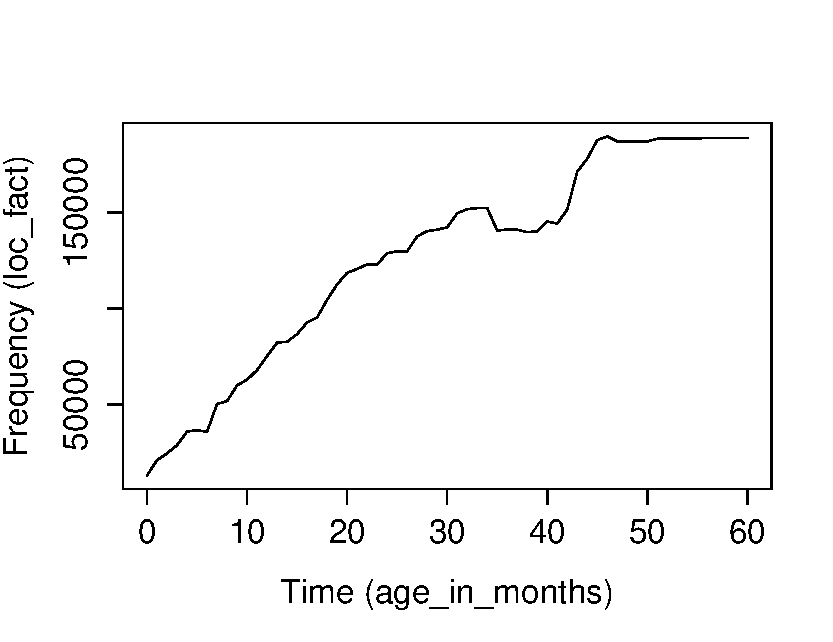
\includegraphics[height=192pt]{images/signal_pid_19012.pdf}
\end{figure}

\paragraph{}
The rationale for choosing 'lines of code' as time series is done because of
its simplicity and intuitive interpretation. Additionally, LOC over time is a
way to measure the growth of the project.

\paragraph{}
The $LOC$ metric used in this study for the transform and analysis is slightly
different from the $loc\_fact$ that is available at Ohloh. The goal for the
signal processing is to be able to detect patterns in a project's code
activity. This means that all changes that occur in source files are of
interest. Therefore, the same metric as in the original study by
\citet{karus2013} is used. The $LOC$ metric is constructed as the sum of
$loc\_fact$, $comments\_fact$, and $blanks\_fact$.

\paragraph{}
For the wavelet transform and analysis, I have used the R Statistics Suite
with packages ``wavelets'', ``chron'', and ``zoo''. The Wavelets package
contains implementations of discrete wavelet transform functions, including
the Haar filter; Chron provides functions for working with chronological data
series; and Zoo eases indexing of and working with indexed data.

The Haar filter is used by \citet{karus2013} because of its simplicity and ease
of interpretation. As this study is a replication of \citeauthor{karus2013}'
study, the choice of using the Haar filter was made.

\paragraph{}
The R scripts used for the steps of wavelet transform, sequence identification,
and grouping, are based on the scripts created and used by
\citeauthor{karus2013} in the initial research. Small adjustments have been
made to make the scripts compatible with the data set.

\subsection{Wavelet transform}
The first step in the analysis of time series of software evolution is the
wavelet transform. During this step discrete wavelet transform using the Haar
filter is applied on a project's signal. The results comprise the
coefficients at each level of decomposition which are saved for further
analysis.

The coefficients are not the same as data points. The data points represent
monthly facts from a project, and the coefficients represent values found at a
certain level of decomposition from the wavelet transform. More specifically:
the coefficients are values resulted from shifting or scaling the signal. For
more details on wavelet transform and analysis see section
\ref{wavelet_analysis}.

\subsection{Wavelet analysis}
\subsubsection{Similar sequence identification}
The coefficients resulting from the wavelet transform are analysed to find
\textit{similar sequences}. A sequence is defined as a series of coefficients
at a particular level of decomposition, with a sequence length between 3 and 65
(inclusive) coefficients.

The sequence length thresholds were chosen by \citet{karus2013} in the original
study to distinguish a sequence from an ordinary set of coefficients if the
sequence is very short (length 1 or 2). Or, in case the sequence is very long,
the ability to distinguish the sequence from the complete signal, hence the
maximum length of 65.

\paragraph{}
In the search for similar sequences, the sequences of one project at a time are
analysed against sequences of other projects. A sequence is considered
'similar' if at least one other sequence was found of which the values of the
coefficients are equal with respect to an allowed deviation of 0.005. This
number is a configuration made by \citeauthor{karus2013} in the original study.
The choice was made to keep it the same in order to get similar results.
A lower or higher value will yield fewer or more similar sequences
respectively.

\paragraph{}
A distinction is made between the \textit{detection} of a sequence and an
\textit{occurrence} of a sequence. Although the difference is slight, the
distinction is needed for further analysis.

A sequence $x$ is \textit{detected} in a project $X$ if it was encountered by
analysing that particular project. Finding an \textit{occurrence} of a sequence
means that a sequence $y$  of another project $Y$ was found to be similar to
sequence $x$ by evaluating that other project's sequences. A sequence is then
recorded as a pair of sequence $x$ detected in project $X$ and a sequence $y$
of project $Y$.

\paragraph{}
The process of finding similar sequences constructs ordered pairs of sequences
from the one project to another. The first entry of the pair is the project
of which the sequence was first discovered (i.e., detected), the second is the
project of the similar sequence (i.e., occurrence). Similar sequences may be
found within one project, but can also be found across projects.\\

\noindent
The properties of a similar sequence are described in Table
\ref{table:sequence_props}.

\begin{table}[H]
\caption{Similar sequence properties}\label{table:sequence_props}
\centering
\begin{tabular}{lp{10cm}}
\hline
	\textbf{Property} & \textbf{Description} \\
	\hline
	Coefficient type & The type of coefficient; either
	W (wavelet/shift), or V (filter/scale). \\
	Project0 & The identity of the project the sequence was detected in. \\
	Project1 & The identity of the project having the similar sequence. \\
	Level0 & The compression level at which the sequence was detected. \\
	Level1 & The compression level at which the similar sequence was found. \\
	Start0 & The index of the coefficient the detected sequence starts. \\
	Start1 & The index of the coefficient at which the similar sequence starts. \\
	Length & The length representing the number of coefficients of the sequence. \\
	Maximum deviation & A number representing the precision of similarity as the
	maximum deviation between coefficients of project0 and those of project1. \\
	Sequence & The list of coefficients representing the sequence of project0. \\
\hline
\end{tabular}
\end{table}

\subsubsection{Similar sequence grouping}
\label{def:pattern}
Not all of the sequences found in the previous step are of equal value. Many of
the sequences considered similar are contingent or represent trivialities. In
the sequence grouping step, the similar sequences are taken as input to find
'patterns'.

\paragraph{}
A sequence is considered a 'pattern' if it appears at least 3 times in the
sequence data. Each pattern is assigned an identification number to be used in
further analysis.

\paragraph{}
This process constructs key-value pairs of sequences having the detected
sequence as key (i.e., the pattern), and a set of similar sequences (i.e.,
occurrences) as value. Additionally, meta data is added to the grouped
sequences. The properties of a pattern, in addition to the sequence properties
from Table \ref{table:sequence_props}, are shown in Table
\ref{table:pattern_props}.

\begin{table}[H]
\caption{Pattern properties}\label{table:pattern_props}
\caption*{\footnotesize\textit{The list of sequence properties also applies to
patterns.}}
\centering
\begin{tabular}{lp{10cm}}
\hline
	\textbf{Property} & \textbf{Description} \\
	\hline
	ID & The identity of the pattern. \\
	Project count & The number of projects containing at least one similar
	sequence. \\
	Occurrences & The number of occurrences of the pattern. \\
	Project list & The list of projects having a similar sequence. \\
	Sequences & The list of similar sequences making the pattern; defined as a list
	of 3-tuples of project ID, level, and start index. \\
	Has dead & A boolean value indicating whether the project list contains at
	least one dead project. \\
	Has alive & A boolean value indicating whether the project list contains at
	least one alive project. \\
\hline
\end{tabular}
\end{table}

\section{Pattern classification}
\label{section:patterns_dead}
Given the dead projects in the data set, all patterns detected in the dead
projects are selected. Patterns detected in dead projects can be hints of
evolutionary events that lead to the death of the project.

The patterns found in dead projects will not occur all at the same moment in
the lifetime of the projects. Therefore, three types of patterns for dead
projects are introduced.

\vspace{1em}
\label{def:pattern_typea}
\begin{description}
	\item[Type A pattern]
		A pattern is a Type A pattern if and only if:
		\begin{itemize}
			\item it is detected in a dead project;
			\item for all occurrences in dead projects, the end of the sequence matches
				the end of the dead project evolution.
		\end{itemize}
\end{description}

\vspace{1em}
\noindent
For example: if the evolution of a dead project $P$ starts at point $x$ and ends
at point $y$, then a type A pattern is detected at point $x'$ and ends at point
$y$ in project $P$.

\vspace{1em}
\label{def:pattern_typeb}
\begin{description}
	\item[Type B pattern]
		A pattern is a Type B pattern if and only if:
		\begin{itemize}
			\item it is detected in a dead project;
			\item for all occurrences in dead projects, the end of the sequence
				\underline{does not} match the end of the dead project evolution.
		\end{itemize}
\end{description}

\vspace{1em}
\noindent
Characterising the patterns according to the above definitions will leave a
group of patterns that \textit{weakly} comply to both definitions.

\vspace{1em}
\label{def:pattern_typeab}
\begin{description}
	\item[Type AB pattern]
		A pattern is a Type AB pattern if and only if:
		\begin{itemize}
			\item it is detected in a dead project;
			\item for some occurrences in dead projects, the end of the sequence matches
				the end of the dead project evolution;
			\item for some occurrences in dead projects, the end of the sequence
				\underline{does not} match the end of the dead project evolution.
		\end{itemize}
\end{description}

\vspace{1em}
\noindent
The above types partition the total set of patterns detected in dead projects
into three disjunctive sets. Although the classification of the patterns into
these types mention only the occurrences in dead projects, the patterns may
occur in alive projects too. However, occurrences in alive projects are not
taken into account for the classification.

\section{Survivability}
\label{section:survivability}
In the search for patterns that are warning signs the patterns of type A will
be the most interesting, because these patterns occur near the end of evolution
of dead projects. These patterns could indicate an evolutionary event that has
lead to the end of code evolution for the dead projects it appears in.

To determine whether the chances for a project to die increase when having a
type A pattern, two groups are made:
\begin{description}
	\item[G0] \quad The group consisting of projects \underline{not} having an
		occurrence of a type A pattern.
	\item[G1] \quad The group consisting of projects having an occurrence of a type
		A pattern.
\end{description}

\noindent
Both groups contain dead and alive projects, are of equal size, and are
disjunct by definition.

The selection of projects for G1 is done by selecting all projects having an
occurrence of a type A pattern. The selection of G0 (i.e., the control group)
is done by using the tool from \citet{nagappan} to make the control group
representative to the whole set of projects.

For each dead project it is recorded at what age the project died. For the
alive projects, the maximum age in the data set is used. The state of 'death' is
taken as event for the Kaplan-Meier estimation of survival function for the
projects.

\begin{comment}
- Execution of the research
- Phases, steps

This chapter reports on the execution of the research method as described in Chapter 3.

If the research has been divided into phases (e.g., using sub questions) the
phases are introduced, reported on and concluded individually. If needed this
Chapter could be split up to balance out the sizes of all Chapters.
An example Research Chapter is provided as Chapter 3 at Paul’s home
page\footnote{http://homepages.cwi.nl/~paulk/thesesMasterSoftwareEngineering/2006/ReneWiegers.pdf}.
\end{comment}
